\subsection{Overview}


\subsection{Functional Requirements}
LuckyCalendar is a calendar system with special functionality allowing users to find new experiences. LuckyCalendar has standard calendar functionality that allows a user to create an appointment, add other users to the appointment and synchronize with GoogleCalendar. LuckyCalendar has a flat-structured user-system, which means that there is no owners of an appointment which allows all normal participants to edit an appointment. \\

In addition LuckyCalendar introduces the functionality of a LuckyAppointment, which allows the user to mark a period of time in her calendar, where she wishes to have an appointment. If another user has made an Appointment with room for LuckyParticipants within the time frame and area, the original user is added to this appointment. A LuckyParticipant does not have rights to edit an appointment, this is the only kind of ownership in the Calendar.\\

Lastly since LuckyCalendar is specialized in its ability to let people make new acquaintances, users might want to use it is a supplement to other calendar systems, therefor LuckyCalendar should be able to synchronize with Google Calendar.


\subsection{Nonfunctional Requirements}				%3_03
	\subsubsection*{}
	{\tabulinesep=1.2mm
\begin{tabu}{ | p{3cm} | p{13cm} |}
    \hline
    Category	 			& 		Requirements \\\hline
    Usability:	  			& 		98\% of the 15-30-year-olds users should be able create, delete, edit appointments and account without prior knowledge, reading or education. \\\hline
    Reliability: 			& 		- Crashes/loss of connection must not cause loss of neither account- or appointment information, none-submitted data may be lost. \\
							&		- It should always be possible to access the server, when the client has Internet connection.\\
							&		- Crashes should be rare - less than 1\% of operations made by a user may lead to a crash. \\ \hline
	Performance:			&		- The system should be scalable - there should only be a hardware limit to the number of appointments or accounts in the system.\\
							&		- The calendar should load fast - there should be a maximum 1-2 second delay on normal computers with 1 mbit connection.\\
							&		- Client should be able to run on a single core 500 MHz CPU.\\ \hline
    Supportability: 		& 		- The system should be documented.  \\
    						&		- Update-able to new browsers and OS'. \\ \hline
	Implementation: 		&		- Requires an Internet connection.\\\hline
	Operation:				&	 	- None. \\\hline
	Legal:					&		- User should agree to terms of use.\\\hline
\end{tabu}
}
\\

\subsection{System models}							%3_04
	\subsubsection{Scenarios}
\textbf{Scenario 1: Create User} \\
	{\tabulinesep=1.2mm
\begin{tabu}{ | p{3cm} | p{13cm} |}
    \hline
    ScenarioName: 			& 		CreateHelleAsUser\\ \hline
    Participating 			& 		\underline{Helle} (User) <initiator> \\	\hline
    Flow of events: 		& 		1. \underline{Helle} wants a calendar system and would like one that could give her new experiences. \\
							&		2. \underline{Helle} opens Calendar and selects create user\\
							&		3. \underline{Helle} enters her email and password.\\
							&		4. \underline{Helle} is created in the system and recieves a notification mail. It is immediately suggested that she creates a \underline{lucky appointment.}\\\hline
\end{tabu}
}
\\\\
\textbf{Scenario 2: Create Appointment} \\
	{\tabulinesep=1.2mm
\begin{tabu}{ | p{3cm} | p{13cm} |}
    \hline
    ScenarioName: 			& 		HelleAndLarsWantsToPlayBingo\\ \hline
    Participating 			& 		\underline{Helle} (User) <initiator> \\
    actors:					&		\underline{Lars} (User) <participant>\\ 
    						&		\underline{Unknown} (User) <LuckyParticipant> \\
    						&		\underline{Calendar} (System) \\	\hline
    Flow of events: 		& 		1. \underline{Helle} and \underline{Lars} wants to play Bingo this Saturday, but they are missing people to play with. \\
							&		2. \underline{Helle} creates an \underline{appointment} (CreateAppointment) for the event. She enters location, time and description, adds \underline{Lars} and makes room for 4 unknown participants\\
							&		3. \underline{Calendar} fills up the \underline{appointment} (MatchAppointment) with LuckyParticipants that matches Helles time and area.\\
							&		4. \underline{Calendar} notifies \underline{Helle} and \underline{Lars} about the Users added to the event, and notifies the Users added to the event with time and place of the appointment.\\
							&		5. One \underline{unknown user} decides to leave the appointment. \\
							&		6. \underline{Calendar} goes over step 3 and 4 again.\\
							&		7. Saturday comes, \underline{Helle} and \underline{Lars} plays bingo with some potentially new friends.\\ \hline
\end{tabu}
}
\\

\pagebreak
\subsubsection{Use case model}
\textbf{UseCases} \\
	
	\begin{center}	
	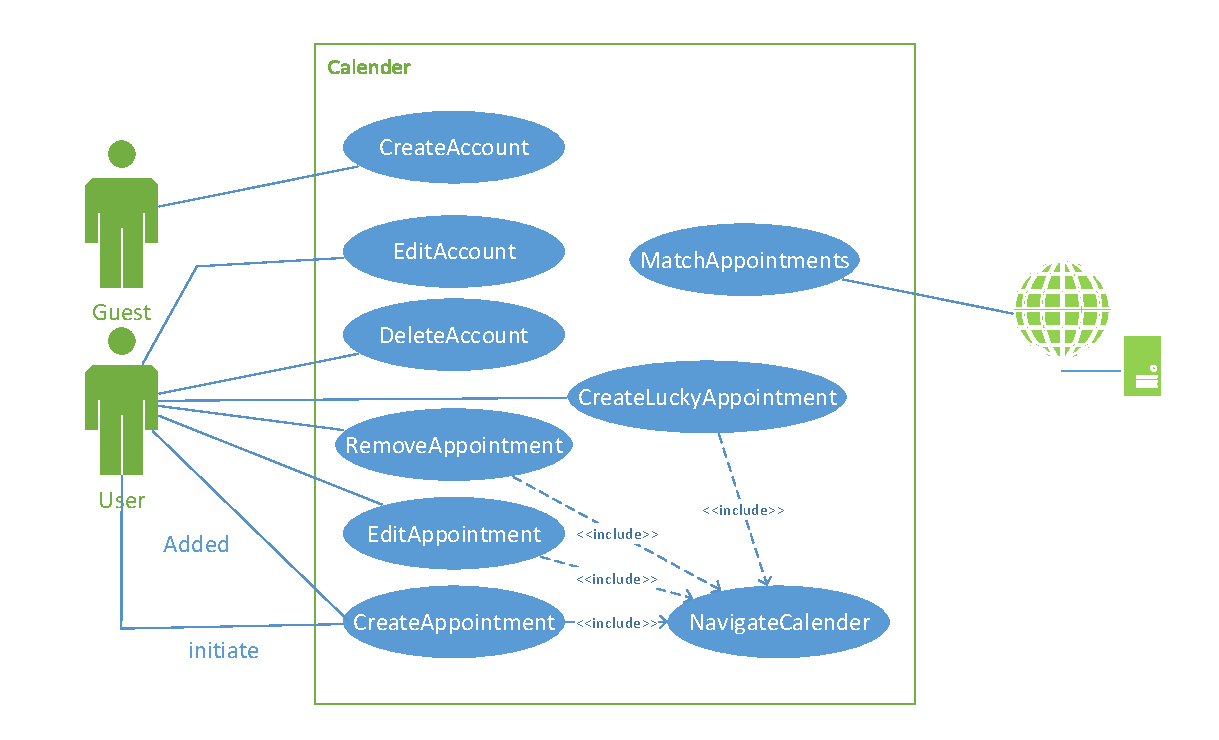
\includegraphics[scale=0.62]{sections/3_04_system_models/UseCaseDiagram.pdf}\\
		{\tabulinesep=1.2mm
\begin{tabu}{ | p{3cm} | p{13cm} |}
    \hline
    Use case name: 			& 		CreateAppointment\\ \hline
    Participating  			& 		User wants to create an appointment with some friends and seeks additional participants. \\
    actors:					&		Users invited to the appointment.\\ \hline
    Flow of events: 		& 		1. User opens Calendar. \\
							&		2. Calendar shows the calendar navigation.\\
							&		3. User selects the date and time of the appointment.\\
							&		4. Calendar shows a form for entering description and place and participants.\\
							&		5. User fills the form, adds participants through email and enters how many additional participants he seeks.\\
							&		6. Calendar creates the appointment and notify participants that they have been added to the event.\\
							&		7. Her er en øndring i denne usacase.\\ \hline
    Entry condition: 		& 		- User is logged in  \\ \hline
	Exit conditions: 		&		- Appointment is changed.\\
							&		- User close the system.\\
							&		- Connection lost.\\\hline
	Quality requirements	&	 	- None \\\hline
\end{tabu}
}\\[1in]
		{\tabulinesep=1.2mm
\begin{tabu}{ | p{3cm} | p{13cm} |}
    \hline
    Use case name: 			& 		CreateLuckyAppointment\\ \hline
    Participating  			& 		User wants to create a lucky appointment. \\
    actors:					&		Users seeking participants.\\ \hline
    Flow of events: 		& 		1. User opens LuckyCalendar. \\
							&		2. LuckyCalendar shows the calendar navigation.\\
							&		3. User selects date and time of the appointment, and that he wishes to make a lucky appointment.\\
							&		4. LuckyCalendar asks in which areas the appointment may take place.\\
							&		5. User selects the areas for the lucky appointment.\\
							&		6. LuckyCalendar creates the appointment and may later inform the user about the appointment he has been matched with.\\ \hline
    Entry condition: 		& 		- User is logged in  \\ \hline
	Exit conditions: 		&		- User account is deleted.\\
							&		- User closes the system.\\
							&		- Connection lost.\\\hline
	Quality requirements	&	 	- None \\\hline
\end{tabu}
}\\[1in]
		{\tabulinesep=1.2mm
\begin{tabu}{ | p{3cm} | p{13cm} |}
    \hline
    Use case name: 			& 		EditAppointment\\ \hline
    Participating  			& 		User wants to edit time and date of an appointment. \\
    actors:					& 		\\ \hline
    Flow of events: 		& 		1. User opens Calender. \\
							&		2. Calender shows the calender navigation.\\
							&		3. User selects the appointment he wants to change.\\
							&		4. Calender shows the appointment in normal mode that allows changes.\\
							&		5. User enters submits the wished changes.\\
							&		6. Calender updates the appointment and notify potential participants about the changes.\\ \hline
    Entry condition: 		& 		- User is logged in  \\ \hline
	Exit conditions: 		&		- Appointment is changed.\\
							&		- User close the system.\\
							&		- Connection lost.\\\hline
	Quality requirements	&	 	- None \\\hline
\end{tabu}
}\\
		{\tabulinesep=1.2mm
\begin{tabu}{ | p{3cm} | p{13cm} |}
    \hline
    Use case name: 			& 		DeleteAccount\\ \hline
    Participating  			& 		User wants to delete her account. \\
    actors:					&		Other users effected by deletion.\\ \hline
    Flow of events: 		& 		1. User opens the program. \\
							&		2. Calendar shows the calendar navigation.\\
							&		3. User selects edit profile.\\
							&		4. Calendar shows the profile edit.\\
							&		5. User select delete account.\\
							&		6. Calendar removes the user from all appointment. If the user was the only participant, the appointment is deleted.\\
							&		7. Calendar deletes account, and notifies other users about changes made to their appointments. \\\hline
    Entry condition: 		& 		- User is logged in  \\ \hline
	Exit conditions: 		&		- User account is deleted.\\
							&		- User close the system.\\
							&		- Connection lost.\\\hline
	Quality requirements	&	 	- None \\\hline
\end{tabu}
}\\[1in]
		{\tabulinesep=1.2mm
\begin{tabu}{ | p{3cm} | p{13cm} |}
    \hline
    Use case name: 			& 		RemoveAppointment\\ \hline
    Participating  			& 		User wants to remove an appointment from his/her calendar. \\
    actors:					&		Other users effected by deletion.\\ \hline
    Flow of events: 		& 		1. User opens LuckyCalendar. \\
							&		2. LuckyCalendar shows the calendar navigation.\\
							&		3. User selects the appointment he wants to remove.\\
							&		4. LuckyCalendar shows the appointment in normal mode that allows changes.\\
							&		5. User selects remove appointment.\\
							&		6. LuckyCalendar remove the event accordingly and notifies other participants. If the user was the last Participant the appointment is deleted from the system.\\\hline
    Entry condition: 		& 		- User is logged in.  \\\hline
	Exit conditions: 		&		- Appointment is deleted.\\
							&		- User closes the system.\\
							&		- Connection lost. (See Use Case "SynchronizeOfflineChanges)\\\hline
	Quality requirements	&	 	- None \\\hline
\end{tabu}
}\\
		{\tabulinesep=1.2mm
\begin{tabu}{ | p{3cm} | p{13cm} |}
    \hline
    Use case name: 			& 		MatchAppointments\\ \hline
    Participating actors:	& 		Calendar is matching appointments missing people with with people seeking appointment. \\
 							&		Users seeking appointment and users looking for appoitnment.\\ \hline
    Flow of events: 		& 		1. Calendar finds all appointments looking for participants. \\
							&		2. For each missing participant Calendar searches for a person seeking an appointment.\\
							&		3. If a match is found, the person is added to the appointment.\\
							&		4. Calendar notifies all users added to an appointment, and user who have an appointment where users are added to. User and appointments where no matches has been found, are notified if they are within a certain timelimit of the appointment.\\\hline
    Entry condition: 		& 		- Calendar runs this procedure x times a day. \\ \hline
	Exit conditions: 		&		- Calendar has looked through all apppointments.\\\hline
	Quality requirements	&	 	- None \\\hline
	Notes					&	 	- We might need a more clever approach, if we as many people getting an appointment as possible \\\hline
\end{tabu}
}\\[1in]
		{\tabulinesep=1.2mm
\begin{tabu}{ | p{3cm} | p{13cm} |}
    \hline
    Use case name: 			& 		NavigateCalendar\\ \hline
    Participating  			& 		User wants to see what he is doing first Friday next month. \\
    actors:					&		Users seeking participants.\\ \hline
    Flow of events: 		& 		1. User opens LuckyCalendar. \\
							&		2. LuckyCalendar shows the a matrix containing the current month. Users appointment are highlighted.\\
							&		3. User selects next month.\\
							&		4. LuckyCalendar shows a similar matrix over the next month.\\
							&		5. User selects the first Friday of the month.\\
							&		6. LuckyCalendar an overview of the day and all the activities. In addition there are buttons for Create Appointment and Create Lucky Appointment.\\ \hline
    Entry condition: 		& 		- User is logged in  \\ \hline
	Exit conditions: 		&		- User closes the system.\\ \hline
	Quality requirements	&	 	- None \\\hline
\end{tabu}
}\\
	\end{center}
	
\subsubsection{Object model}
		\input{sections/3_04_system_models/OM_Entities}\\[1in]
	\begin{center}	
		\input{sections/3_04_system_models/OM_Control}\\[.2in]
		\input{sections/3_04_system_models/OM_Boundary}\\
	\end{center}
			\begin {figure}
	\textbf{Class Diagram}
	\center{
	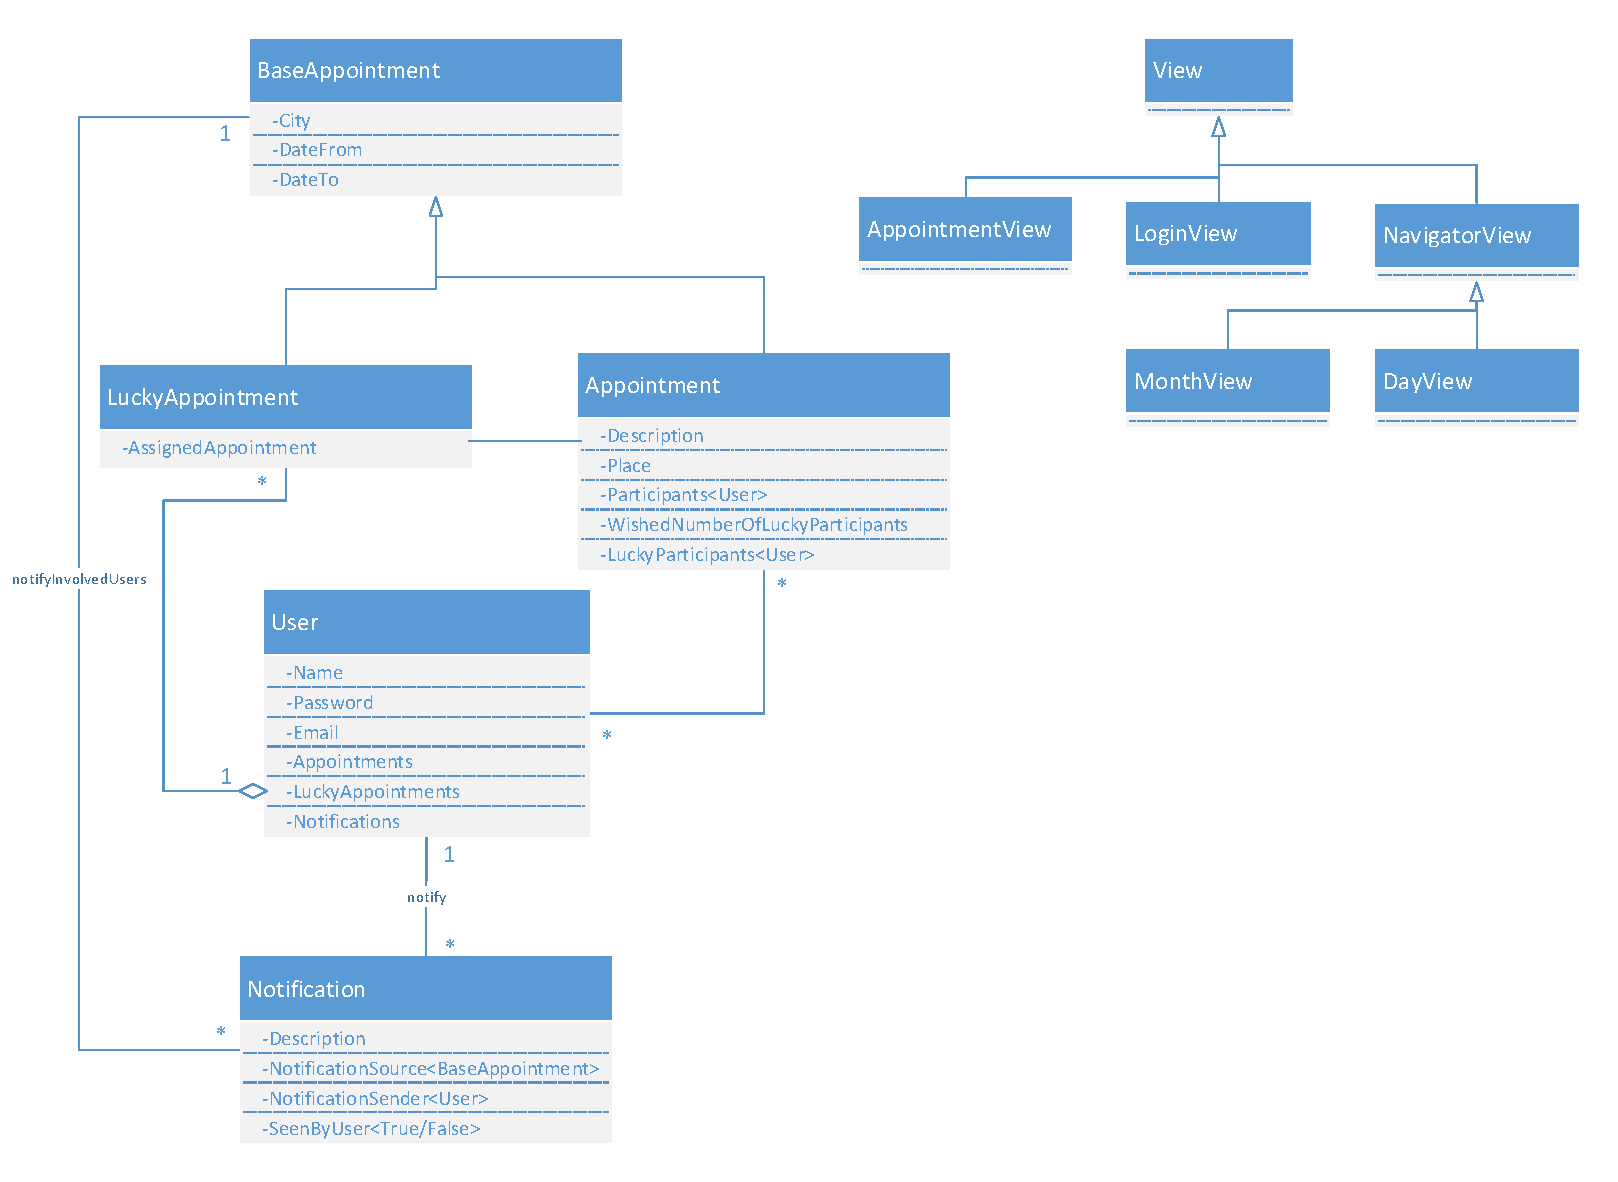
\includegraphics[scale=0.65]{sections/3_04_system_models/ClassDiagram.pdf}
	}
	\caption{Notice how the LuckyAppointment has only one user - this is due to the fact that a LuckyAppointment is an Appointment where one user has left time free for being added to anothers appointment}
	\end{figure}

	\pagebreak

\subsubsection{Dynamic model}

	\paragraph{Sequence Diagram: Create Appointment Seeking Participants} 
	\center{
	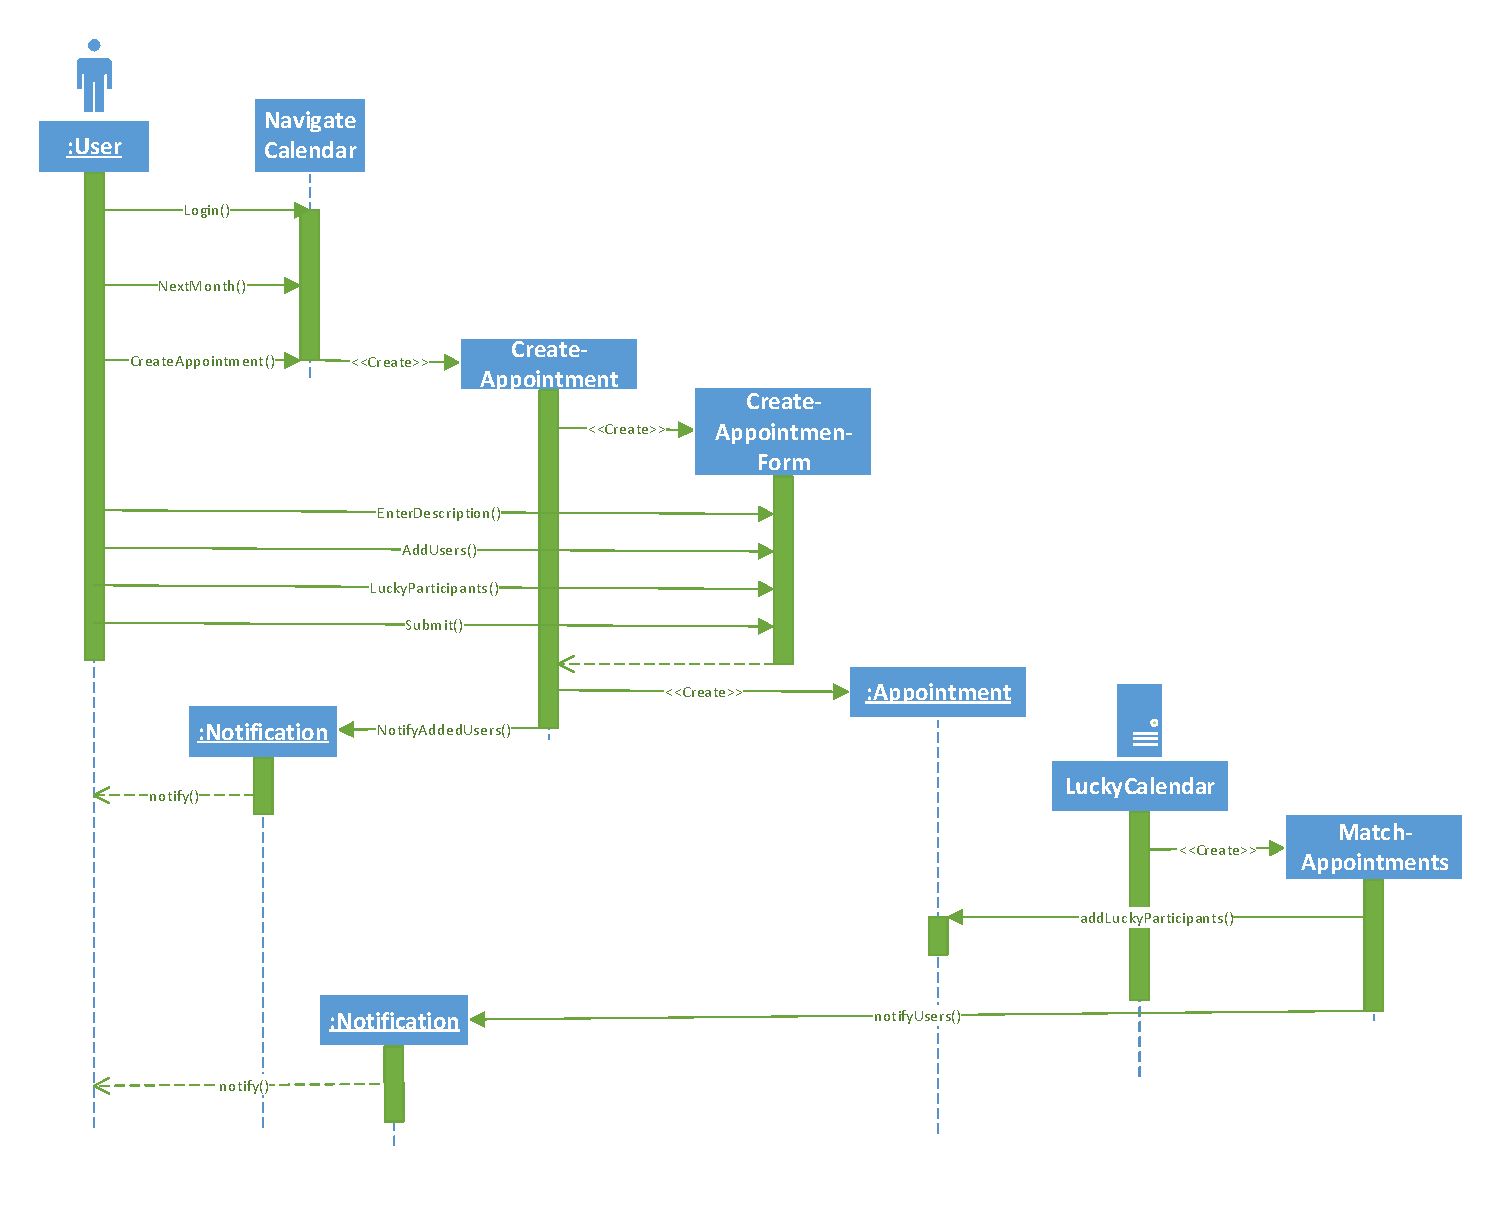
\includegraphics[scale=.7]{sections/3_04_system_models/SQ_CreateAppointment.pdf}
	}
	\pagebreak

	\paragraph{State Machine Diagram: States of appointment}
	\center{
	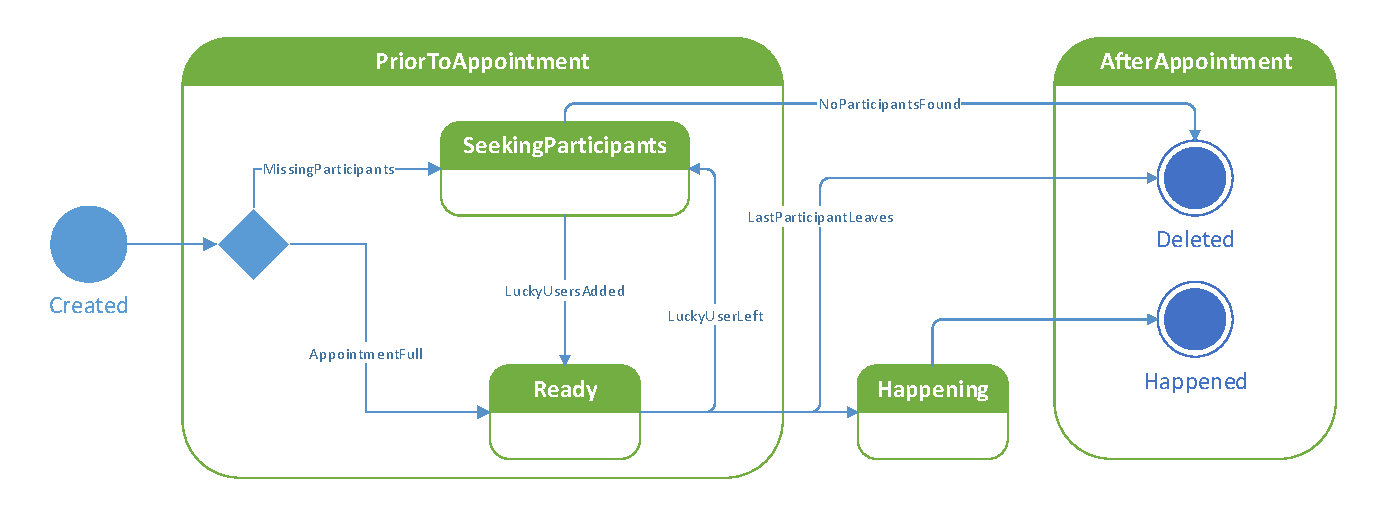
\includegraphics[scale=.7]{sections/3_04_system_models/SM_Appointment.pdf}
	}
\subsubsection{User interface}

\